
\newcommand{\etas}{\ensuremath{\eta_{\mathrm{s}}}}


\chapter{Background and Introduction}

\section{Stratospheric Airships}
In the present climate of growth in broadband-hungry telecommunication applications, wireless infrastructure providers are under continuous pressure to exploit the limited radio spectrum as efficiently as possible. In this context, high altitude platforms (HAPs) are increasingly being cited as having an important role to play in future systems and applications. They have the potential to exploit many of the best aspects of terrestrial and satellite based systems, while offering advantageous propagation characteristics. Such platforms may be airships or aircraft and for environmental considerations would ideally be solar powered.
\begin{figure}[htbp]
	\centering
	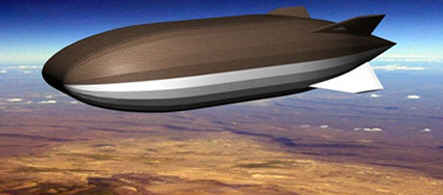
\includegraphics{intro/Stratellite.jpg}
	\caption{A stratospheric airship (Stratellite)}
	\source{Source: http://www.virtualworldlets.net}
	\label{Stratellite} %      only if needed 
\end{figure}

Keeping the above problem in mind, a stratospheric airship can be designed which can float at an altitude of 17-25 km and would be powered by direct solar energy extracted by photo-voltaic cells during day time and energy stored in the regenerative fuel cells during night time. The airship is required to stay aloft at a particular position despite of the wind gusts. So,the position should be corrected from time to time. This demands for the need of propellers using which the position of the airship at a particular altitude is corrected from time to time.

17-25 KM altitude is the place where little or no weather activities like rain, thunderstorms or cyclones takes place. At that altitude, things like pressure, density temperature and wind velocity remains constant or changes from season to season. So, this layer can be utilized to station our stratospheric airship.

 There are potentially many advantages of stratospheric airships compared to ground level telecommunication or satellite communication systems. Some of them are:
 
 \begin{itemize}
 	\item Larger ground coverage compared to ground level telecommunication systems like towers.
 	\item They can be used for strategic surveillance purposes by defence and military agencies.
 	\item They can be thought of an alternative to geostationary satellites with two potential advantages. One being low initial and operating costs involved. Second being the ability to update, repair and maintain the payload systems from time to time.
 	\item They can be used for communication purposes during emergency caused because of natural calamities or disasters since ground based telecommunication systems might not work properly at these times.
 \end{itemize}
 
\section{Motivation}

Unconventional non-axisymmetric shapes provides many advantages over conventional axisymmetric shapes for stratospheric airships because they can have flatter upper surface and is advantageous for capturing more solar irradiance. Existing literature has good amount of work on CFD analysis of axisymmetric shapes. But there is no considerable amount of analysis on non-axisymmetric shapes. The reason is obvious, 2D analysis can be easily done for axisymmetric shapes. But to do CFD analysis on non-axisymmetric shapes, we need to perform 3D CFD analysis. 3D analysis demands more computational effort which might not be available for many researchers.

There are many advantages for OpenFOAM\textsuperscript{\textregistered} like availability of source code, small size code (only 200 MB) and complete flexibility in usage. OpenFOAM\textsuperscript{\textregistered} also comes with an inbuilt meshing (\textit{Block mesh} and \textit{Snappy Hex Mesh}) and post-processing (\textit{Paraview}) utilities, both of which are known for their unique and advanced method of problem solving capabilities. \\

\section{Objective and Aims}
The project is divided into two stages namely Stage-1 and Stage-2. In Stage-1, existing CFD results available in the literature for four standard shapes will be reproduced by carrying out 3D CFD analysis using OpenFOAM\textsuperscript{\textregistered}. A methodology for carrying out multi-disciplinary optimization will be laid out. The methodology should be such that optimal shape of the envelope should be obtained in minimum amount of time and optimally utilizing computational resources. The objectives for Stage-2 are explained in Chapter \ref{future plan}

\section{Report layout}
\label{layout}

After providing a brief introduction to Stratospheric Airships outlining the aims and objectives of this study, Chapter \ref{literature} gives the detailed literature survey of various fields required for multi-disciplinary shape optimization. Chapter \ref{geometry}  explains two of the many methods used for the parameterization of geometry. This is also shown in Figure \ref{Report layout}. Next, short introduction for advantages of using OpenFOAM\textsuperscript{\textregistered} is discussed in Chapter \ref{openfoam}. 

Mesh generation using two utilities namely \textit{Gmsh} and \textit{SnappyHexMesh} are discussed in Chapter \ref{mesh}. A brief introduction of methodology for optimization is given in Chapter \ref{optimization}. However optimization will be done in stage -02 along with other considerations as shown in \ref{Report layout}. 

Finally, Chapter \ref{results} discusses the results obtained while validating the results present in literature for various standard airship shapes using OpenFOAM\textsuperscript{\textregistered}. Chapter \ref{future plan} gives the future work that will be performed in stage -02. The workflow for the total project is shown in Figure \ref{Report layout}. The blocks present in transparent oval is the work completed in stage 1. 

\begin{figure}[htbp]
	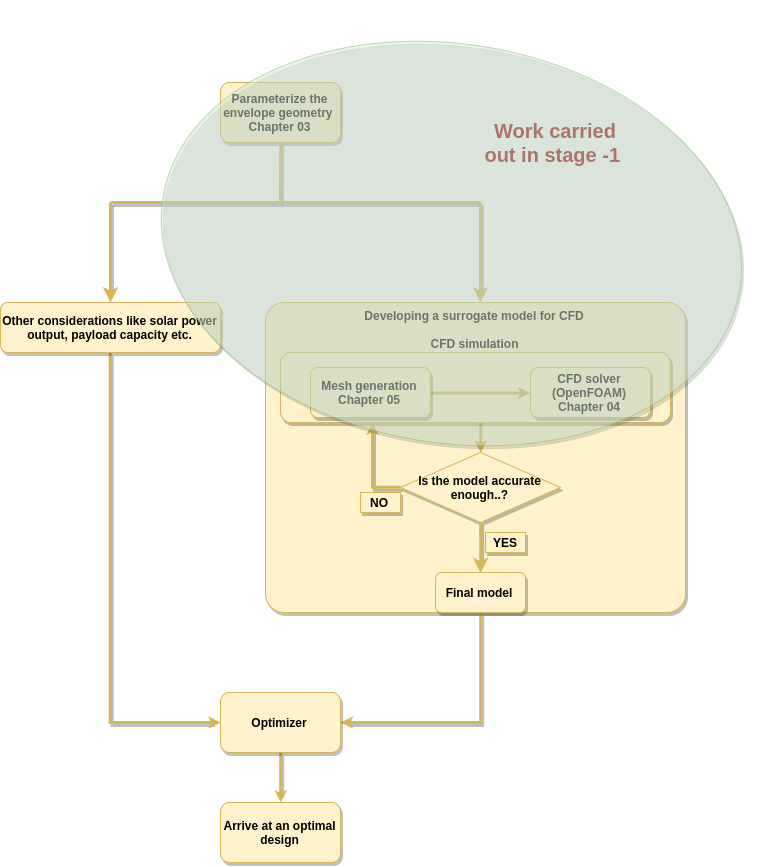
\includegraphics[width=\textwidth]{layout/layout.png} 
	\caption{Work flow of multi-disciplinary shape optimization}
	\label{Report layout} %      only if needed 	
\end{figure}
%%
Next Chapter gives brief literature survey that has been carried out to understand the previous research carried out in the field of High Altitude Airships (HAA's).


%%% Local Variables: 
%%% mode: latex
%%% TeX-master: "../mainrep"
%%% End: 

%%


%%% Local Variables: 
%%% mode: latex
%%% TeX-master: "../mainrep"
%%% End: 
